% !TeX spellcheck = en_US
% !TeX encoding = UTF-8
% !TeX root = ../thesis.tex

\chapter{Evaluation}
This chapter will introduce the setup for the experiments and the tasks.

\section{Setup}
All algorithms were implemented in python,
the optimization algorithm for MORE is Low-storage BFGS
from nlopt\footnote{\href{https://nlopt.readthedocs.io/en/latest/}{https://nlopt.readthedocs.io/en/latest/}}.
The clusterwork2 (cw2) framework, developed at the ALR group, was used for running experiments.
The experiments were conducted on a machine with two 8-core
AMD Ryzen 2700X processores clocked at 2.6 GHz and 31GB of RAM.

- code is uploaded to gitlab/github (archive repo)

\subsection{Hyperparameter search}
We did a mixture of manual hyperparameter search and grid search
with the cw2 framework. At a later stage we incorporated optuna
for hyperparameter optimization.

\section{Experiments}
We now evaluate the performance of our algorithms on various problems.

\subsection{Test Functions for Optimization}
Based on \citet{molga2005test}.

\Cref{fig:rosenbrock} shows the rosenbrock function, a uni-model optimization function. The global minimum $f(\mathbf{x}) = 0$. In the experiments
the mean of the initial distribution has been chosen randomly.

$$ f(x) = \sum^{n-1}_{i=1} [100(x_{i+1} - x_i^2)^2 + (1-x_i)^2] $$

\begin{figure}[ht!]
    \centering
    \includesvg[width=0.5\textwidth]{figures/rosenbrock}
    \caption{rosenbrock function}
    \label{fig:rosenbrock}
\end{figure}

In figures \Cref{fig:5dim} and \Cref{fig:15dim} we show the best results
achieved on 5 dimensional and 15 dimensional rosenbrock. We observe that
the our RLS approach uses the least amount of samples. For 5 dimensional
rosenbrock the BLR approach is ommitted due to considerably worse
performance.
One observation to make is that RLS converges only to around 1e-9, while
the LS approach manages to 
\begin{figure}[ht!]
     \centering
     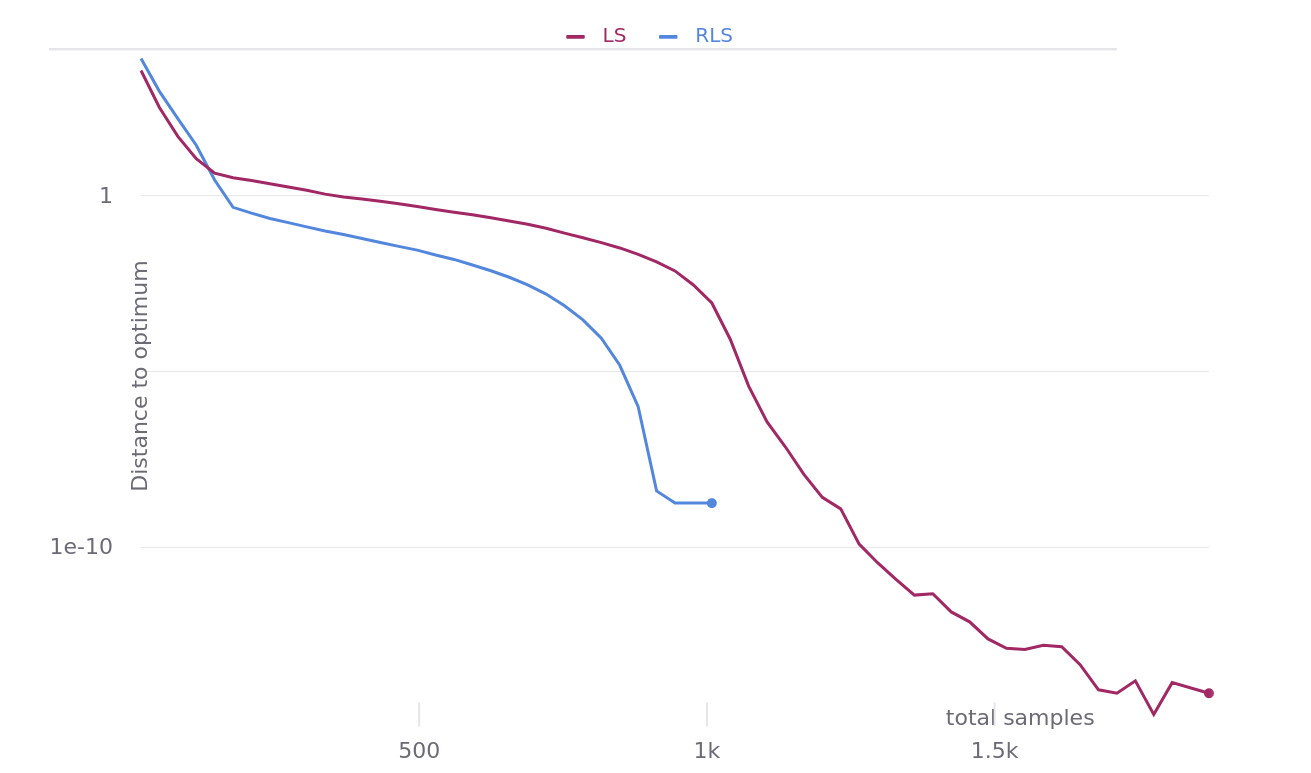
\includegraphics[width=1\textwidth]{figures/5dim}
     \hspace{1cm}                       
     \caption{This figure shows the median of (10 runs) for RLS and LS on 5 dimensional Rosenbrock}
     \label{fig:5dim}
\end{figure}

\begin{figure}[ht!]
     \centering
     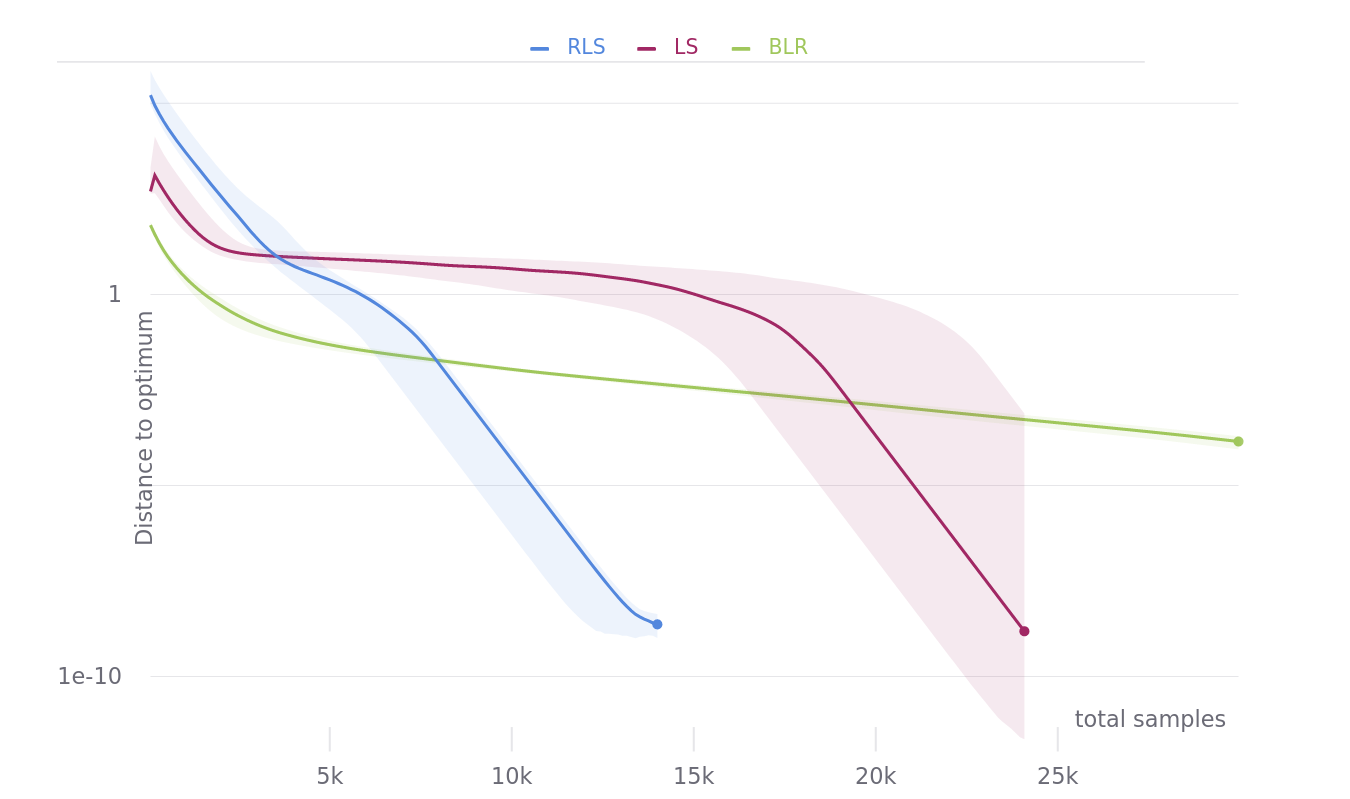
\includegraphics[width=1\textwidth]{figures/15dim}
     \hspace{1cm}                       
     \caption{This figure shows the median of (10 runs) for RLS, LS and BLR (original MORE) on 15 dimensional Rosenbrock}
     \label{fig:15dim}  
\end{figure}

% minipage example
%\begin{figure}
%    \centering
%    \begin{minipage}{0.45\textwidth}
%      \centering
%      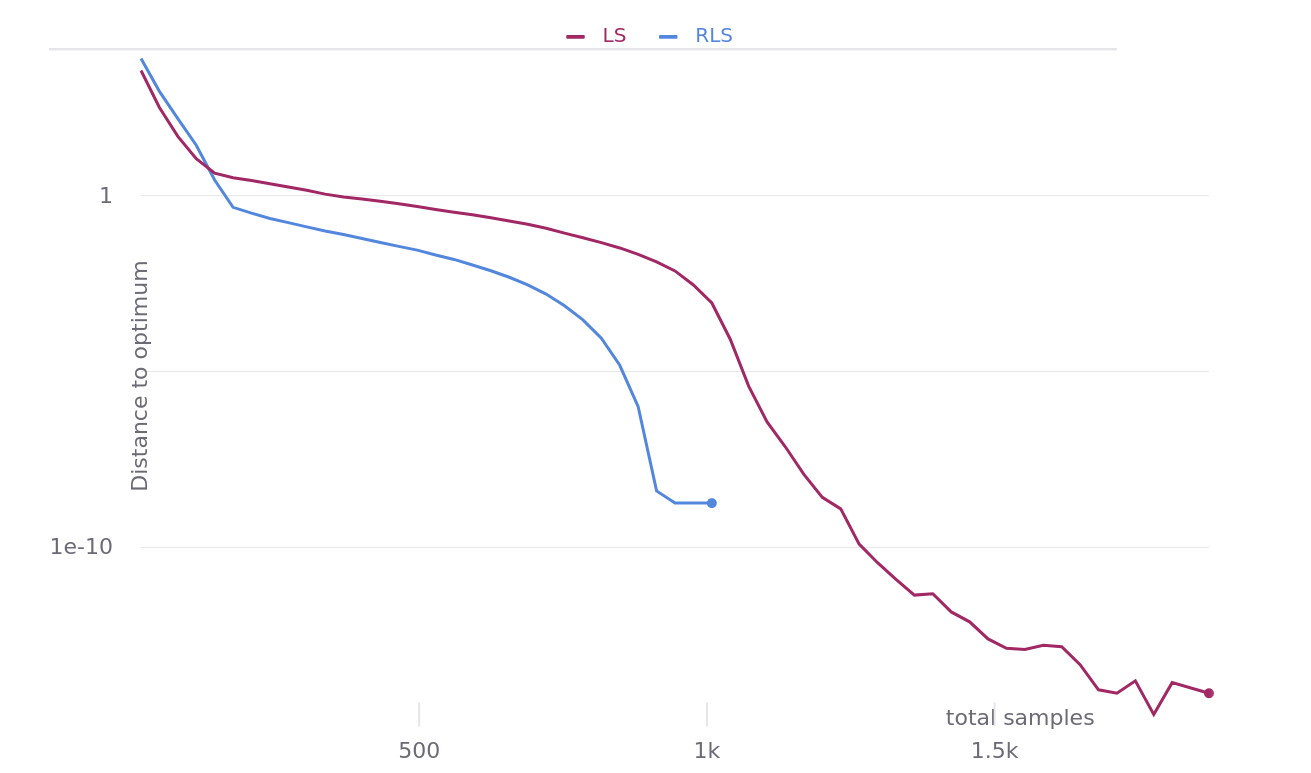
\includegraphics[width=1\textwidth]{figures/5dim}
%      \hspace{1cm}                       
%      \caption{5 dimensional Rosenbrock}
%      \label{fig:5dim}
%    \end{minipage}\hfill
%    \begin{minipage}{0.45\textwidth}
%      \centering
%      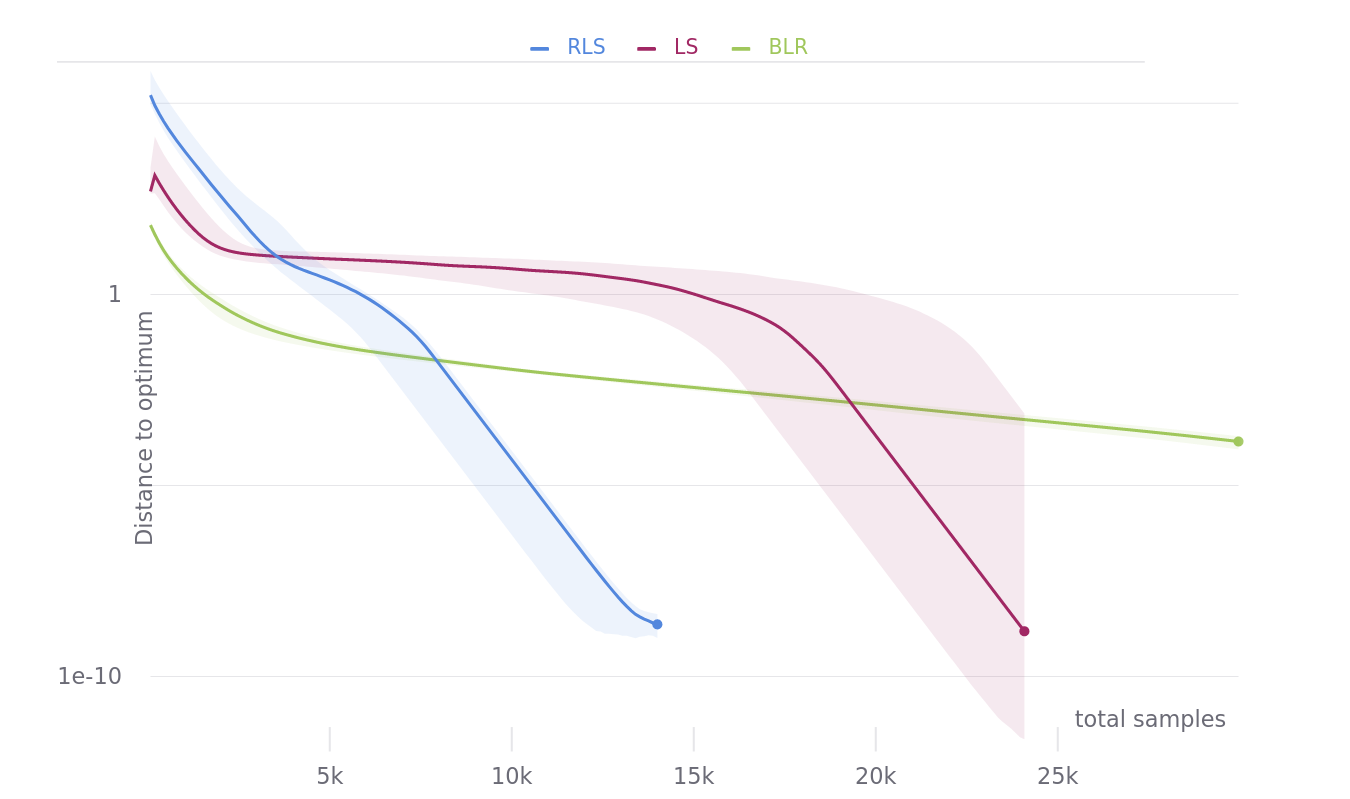
\includegraphics[width=1\textwidth]{figures/15dim}
%      \hspace{1cm}                       
%      \caption{15 dimensional Rosenbrock}
%      \label{fig:15dim}
%    \end{minipage}
%  \end{figure}

\subsection{Planar Reaching Tasks}

\subsubsection{Dynamic Movement Primitives}
- dynamic system-based motor primitives based on work [Ijspeert 2002, Schaal 2003,2007]
improved imitation and reinforcementlearning

- represent both discrete point-to-point movements as well as rhythmic motion
with motor primitives

- first system canonical system (phase variable)

- we can build complex motor skills from basic primitives,
  its based on dynamical systems

- discrete movement primitives using only a single first order system

- key advantage the second system is linear in the shape parameters and can
  be efficiently learned

- initialized with imitation learning

- DMPs as policy representation

\subsection{Via Point Reaching Task}
We used a 5 link robot, similar to MORE setup.
Therefore 25 dimensions of the problem, which should be at viapoint (1,1)
at time step 100 and at viapoint (5,0) at timestep 200.
In \Cref{fig:blr_via} we see the task solved by the original MORE algorithm.

\begin{figure}[ht!]
  \centering
     \includesvg[width=0.6\textwidth]{figures/blr_via}
     \hspace{1cm}                       
     \caption{This figure shows the movement resulting from the policy
       learned by BLR for the viapoint reaching task.
       The postures of the resulting motion are shown as overlay,
       where darker postures indicate a posture which
       is close in time to the hole.}
     \label{fig:blr_via}  
\end{figure}

\subsection{Hole Reaching Task}
5 link robot, that has to reach into hole at [2,0] without collision
with ground or walls.

\subsection{Tests for Preprocessing Methods}
- TODO: place this into appendix?

Tests on data preprocessing methods, different normalization techniques.
Whitening very important, making it possible to track the model parameters
more easily.

- compare normalization techniques (moving average, batch normalization)

- best performance comparison (more iterations)

- best performance comparison of different methods (total samples)

- test influence of KL bound

- test influence of whitening, normalization?

- test influence of noise of drift model

\section{Evaluation}
- some theoretical problems: sample pool, model noise

- improve sample efficency of rosenbrock and reaching task,
better than original MORE and beating CMA-ES benchmark

